%section 2 Status of the transition to dual-stack storage
% sub-section a) Tier 0 and Tier 1's  (Bruno)
% sub-section b) Tier 2's  (Andrea)
% sub-section c) LHCOPN & LHCONE  (Bruno)
% sub-section d) WLCG Data Transfers (Dave)

% Do we start with a few general words of introduction about the general aims and history of the transition to dual-stack storage?
% Together with reminders of the agreed timetable (and refer to old CHEP papers from our group)?

The long process of enabling the protocol IPv6 at LHC started already 10 years ago in 2010. Today, after extensive testing by the HEPiX IPv6 Working Group \cite{ipv6chep2015} and the strong support of the storage developer community, the current WLCG storage and grid-middleware applications fully support the use of IPv4 and IPv6 protocols simultaneously; they are dual-stack ready or even protocol agnostic.


% Subsection '2a'
% Tier 0 and Tier 1's
%
%\subsection{Deployment at the Tier-0 and Tier-1 sites}
\subsection{Deployment at Tier-0 and Tier-1's}
After the aforementioned ten years the storage environment is almost completely dual-stack ready. At the CERN WLCG Tier-0 and at the 14 Tier-1s, dual-stack IPv6/IPv4 is nearly fully enabled. Only the Tier-1 site at the Kurchatov Institute in Moscow, part of the Russian Federation, is still currently running on IPv4-only. This enables a total of 96\% of the Tier-1 storage of WLCG to be accessible via IPv6 as shown in table~\ref{tab:t012stor}.
\begin{table}[h]
\centering
\caption{Fraction of Tier-1 and Tier-2 storage available over IPv6}
\label{tab:t012stor}
\begin{tabular}{lccccc}
\hline
& ALICE & ATLAS & CMS & LHCb & Global \\\hline
Tier-1 storage & 78\% & 96\% & 100\% & 94\% & 96\% \\
Tier-2 storage & 86\% & 59\% &  89\% & 75\% & 74\% \\\hline
\end{tabular}
\end{table}

The FTS server at FNAL is still currently running in IPv4 preferred mode. There was a long-standing malfunctioned transfer issue to IPv4-only Tier-2 sites in the USA which is now solved. This last server will be deployed in dual-stack in the near future.

\subsection{Deployment at Tier-2 sites}
The deployment of IPv6 at Tier-2 sites is still proceeding even after the
official deadline expired at the end of 2018. It was decided not to
give the deadline a formal extension, but just to encourage all
remaining sites to complete the IPv6 deployment ``as soon as
possible'': the main motivations were that \emph{a)} sites behind
schedule were encountering objective difficulties and \emph{b)} the
most effective deadline would be imposed by the experiments
themselves, if they wished, for example, to require IPv6 for
production. This choice was confirmed by the steady progress observed
during 2019, as it can be seen in figure~\ref{fig:t2depl}.
\begin{figure}[h]
\centering
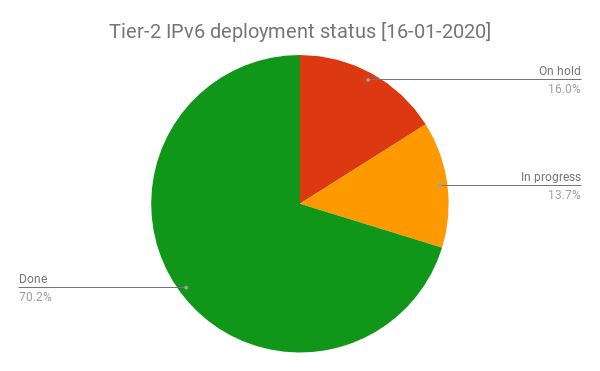
\includegraphics[width=6cm]{chart2}
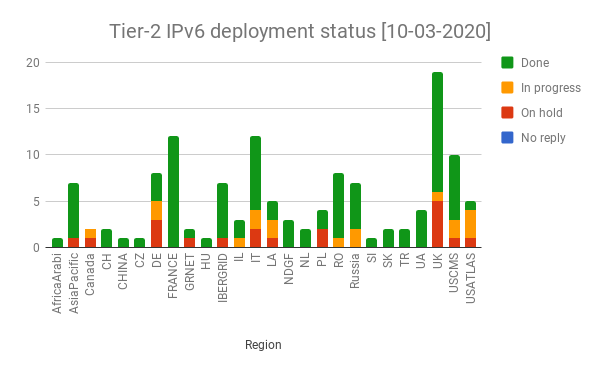
\includegraphics[width=6cm]{chart}
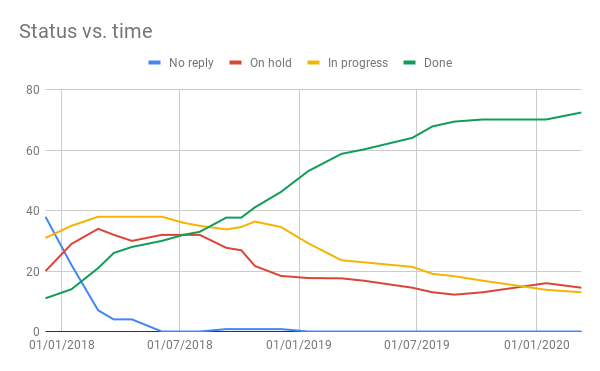
\includegraphics[width=6cm]{chart3}
\caption{(left) Tier-2 deployment status by site globally, (right) by region, and (bottom) time evolution}
\label{fig:t2depl}
\end{figure}

The time evolution of the site status shows a steady increase of the
number of sites that have deployed IPv6, until a more recent
slowdown. This is consistent with the hypothesis that the remaining
sites are those facing the biggest difficulties. A detailed analysis
of the tickets shows that, in many cases, sites need to wait for the
IPv6 deployment on site, which often depends on people different from
the WLCG site staff. The fraction of the Tier-2 storage that is
accessible via IPv6 is shown in table~\ref{tab:t12stor} for each
experiment, and significant differences are apparent.
\begin{table}[h]
\centering
\caption{Fraction of Tier-1 and Tier-2 storage available over IPv6}
\label{tab:t12stor}
\begin{tabular}{lccccc}
\hline
& ALICE & ATLAS & CMS & LHCb & Global \\\hline
Tier-1 storage & 78\% & 96\% & 100\% & 94\% & 96\% \\ 
Tier-2 storage & 86\% & 59\% &  89\% & 75\% & 74\% \\\hline
\end{tabular}
\end{table}
Two experiments (ALICE and CMS) are very close to having all their
Tier-2 storage on IPv6, LHCb has little Tier-2 storage to begin with
due to their particular computing model and ATLAS is getting better,
but still far from the goal.


\subsection{LHCOPN and LHCONE}

The LHCOPN and LHCONE are both virtual private networks (VPN) serving the Large Hadron Colider Experiments. Both networks are from the end of 2016 onward dual-stack ready. LHCOPN is a CERN (Tier-0) centric star network mainly deployed for the distribution of the raw detector data to the Tier-1 sites. Since the majority of Tier-1 sites are dual-stack ready and even while the protocol IPv6 is preferred it is still not the situation that IPv6 is the only transfer protocol, but a tendency towards IPv6 file transfers are recognizable. LHCONE is a network of close to 140 sites connected trough Virtual Routing and Forwarding implementations at 26 different network service providers (NSP). All connected end sites deploying a Border Gateway Protocol (BGP) routing table and advertising their own Classless Inter-Domain Routing (CIDR) to the connecting NSP. The network itself is already since long IPv6 ready. The connected end sites are becoming more and more IPv6 ready. This is recognizable at the  transfer protocol changes from IPv4 towards IPv6. The high usage of the IPv4 transfer protocol visualizes that the fraction of IPv4 only sites is still quite substantial.

%section{File Transfers

\subsection{File transfers}

Over the last 2 years we have been regularly tracking the fraction of WLCG file transfers that take place over IPv6.
(needs more description).

The fraction of data transfers over FTS on IPv6 as a function of date is shown in  figure~\ref{fig:FTS}.
\begin{figure}[h]
\centering
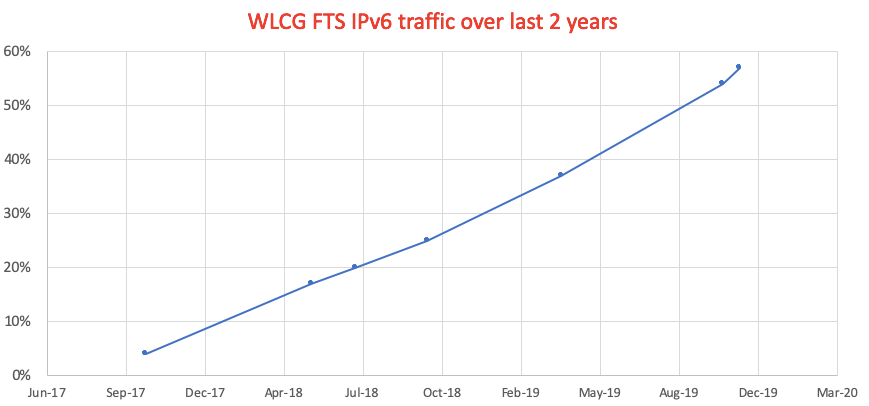
\includegraphics[width=10cm]{FTS}
\caption{Percentage of FTS data transfers over IPv6}
\label{fig:FTS}
\end{figure}


%% Subsection '2a'
% Tier 0 and Tier 1's
%
Some efforts were made to investigate whether the WLCG software packages could be enabled to run in a dual-stack environment or even become protocol agnostic. The first software packages that were examined were data transfer software packages like FTS and SRM. After the examination some software packages were replaced like AFS with EOS, or CASTOR with DPM. Today the storage environment is dual/stack ready and at CERN the Tier-0 is IPv6 and IPv4 dual-stack is enabled. The Tier-1 sites: CA-Triumf, DE-KIT, ES-PIC, FR-CCIN2P3, IT-INFN-CNAF, NDGF, NL-T1 (SARA-Matrix and NIKHEF), RRC-JINR-T1, TW-ASGC, UK-T1-RAL, US-T1-BNL, US-T1-FNAL are dual-stack deployed as shown in the following figure. ~\ref{fig:t1ds}.
\begin{figure}[t]
\centering
%\includegraphics[width=13cm]{Tier-1-IPv6-dual-stack}
\includegraphics[width=13cm]hepix-ipv6-tier01-dual-stack.png}
%\includegraphics[width=13cm]{t1ds}
\caption{Tier-0/1 IPv4/6 dual-stack redyness incl dual-stack perfsonar server deployment}
\label{fig:t1ds}
\end{figure}

But even while the IPv6 redeaness deadline in April 2018 is long ago, there is one part of the russian Tier-1 RRC-KI-T1 still deployed with IPv4 only. The dual-stack perfsonar server is deployed at almost all sites except NL-T1-NIKHEF and RRC-KI-T1. The FTS server at FNAL is still running in IPv4 prefered mode. There were a long standing malfunctioned transfer issue to IPv4 only US-Tier-2 sites which is solved now. This last server will get deployed in dual-stack as soon as possible.   

%\subsection{Deployment at Tier-2 sites}
The deployment of IPv6 at Tier-2 sites is still proceeding even after the
official deadline expired at the end of 2018. It was decided not to
give the deadline a formal extension, but just to encourage all
remaining sites to complete the IPv6 deployment ``as soon as
possible'': the main motivations were that \emph{a)} sites behind
schedule were encountering objective difficulties and \emph{b)} the
most effective deadline would be imposed by the experiments
themselves, if they wished, for example, to require IPv6 for
production. This choice was confirmed by the steady progress observed
during 2019, as it can be seen in figure~\ref{fig:t2depl}.
\begin{figure}[h]
\centering
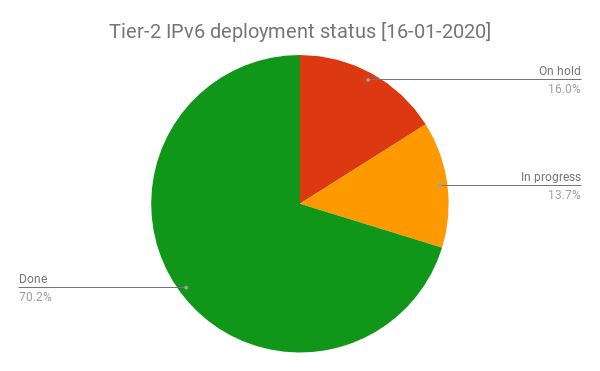
\includegraphics[width=6cm]{chart2}
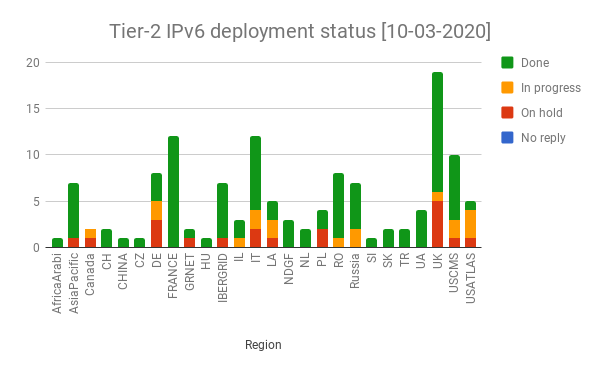
\includegraphics[width=6cm]{chart}
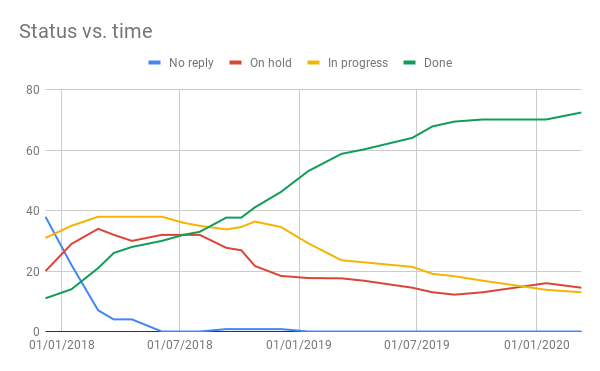
\includegraphics[width=6cm]{chart3}
\caption{(left) Tier-2 deployment status by site globally, (right) by region, and (bottom) time evolution}
\label{fig:t2depl}
\end{figure}

The time evolution of the site status shows a steady increase of the
number of sites that have deployed IPv6, until a more recent
slowdown. This is consistent with the hypothesis that the remaining
sites are those facing the biggest difficulties. A detailed analysis
of the tickets shows that, in many cases, sites need to wait for the
IPv6 deployment on site, which often depends on people different from
the WLCG site staff. The fraction of the Tier-2 storage that is
accessible via IPv6 is shown in table~\ref{tab:t12stor} for each
experiment, and significant differences are apparent.
\begin{table}[h]
\centering
\caption{Fraction of Tier-1 and Tier-2 storage available over IPv6}
\label{tab:t12stor}
\begin{tabular}{lccccc}
\hline
& ALICE & ATLAS & CMS & LHCb & Global \\\hline
Tier-1 storage & 78\% & 96\% & 100\% & 94\% & 96\% \\ 
Tier-2 storage & 86\% & 59\% &  89\% & 75\% & 74\% \\\hline
\end{tabular}
\end{table}
Two experiments (ALICE and CMS) are very close to having all their
Tier-2 storage on IPv6, LHCb has little Tier-2 storage to begin with
due to their particular computing model and ATLAS is getting better,
but still far from the goal.


%\subsection{LHCOPN and LHCONE}

The LHCOPN and LHCONE are both virtual private networks (VPN) serving the Large Hadron Colider Experiments. Both networks are from the end of 2016 onward dual-stack ready. LHCOPN is a CERN (Tier-0) centric star network mainly deployed for the distribution of the raw detector data to the Tier-1 sites. Since the majority of Tier-1 sites are dual-stack ready and even while the protocol IPv6 is preferred it is still not the situation that IPv6 is the only transfer protocol, but a tendency towards IPv6 file transfers are recognizable. LHCONE is a network of close to 140 sites connected trough Virtual Routing and Forwarding implementations at 26 different network service providers (NSP). All connected end sites deploying a Border Gateway Protocol (BGP) routing table and advertising their own Classless Inter-Domain Routing (CIDR) to the connecting NSP. The network itself is already since long IPv6 ready. The connected end sites are becoming more and more IPv6 ready. This is recognizable at the  transfer protocol changes from IPv4 towards IPv6. The high usage of the IPv4 transfer protocol visualizes that the fraction of IPv4 only sites is still quite substantial.


